\documentclass[11pt,a4paper]{article}

% ─── Packages ────────────────────────────────────────────────────────────
\usepackage[utf8]{inputenc}
\usepackage[T1]{fontenc}
\usepackage{amsmath,amssymb,bm}
\usepackage{graphicx}
\usepackage{booktabs}
\usepackage{siunitx}
\usepackage[margin=2.5cm]{geometry}
\usepackage{hyperref}
\usepackage{cleveref}
\usepackage{caption,subcaption}
\usepackage{xcolor}
\usepackage{enumitem}
\usepackage{mathtools}

% ─── Custom commands ─────────────────────────────────────────────────────
\newcommand{\alphag}{\alpha_{\mathrm{g}}}
\newcommand{\Vz}{V_z}
\newcommand{\ERMS}{E_{\mathrm{RMS}}}
\newcommand{\dd}{\mathrm{d}}

% ─── Title ───────────────────────────────────────────────────────────────
\title{%
	Accuracy of Rise Velocity Estimation from Lagrangian Particle Tracking
	Data: \\[4pt]
	A Comparative Analysis of Scattered and Interpolated Approaches}
\author{}
\date{}

\begin{document}
	\maketitle
	
	A systematic numerical analysis has been conducted to assess the accuracy of
	bubble rise velocity estimation from Lagrangian particle tracking data,
	using a 2D axisymmetric rising bubble at $\mathrm{Re}=100$,
	$\mathrm{Bo}=100$ as the test case.  The analysis considered two rise
	velocity definitions (centroid-based and volume-averaged), two data
	representations (scattered and re-interpolated), and four interpolation
	scheme combinations for the gas fraction and velocity fields.
	
	The centroid-based rise velocity consistently outperforms the
	volume-averaged method, with RMS errors that are generally smaller. This superior accuracy is attributed to the
	centroid method's exclusive dependence on the gas fraction field, which is
	interpolated more faithfully than the velocity field during particle
	tracking.
	
	Re-interpolation of scattered Lagrangian data onto a fixed Eulerian grid
	dramatically improves centroid-based estimates but
	offers limited benefit for the volume-averaged method, whose accuracy is
	fundamentally constrained by velocity field interpolation errors.
	
	The dominant source of error in the Lagrangian framework is the velocity
	field interpolation, as confirmed by direct comparison of gas fraction and
	velocity profiles along diagnostic cut-lines.  This observation motivates
	the use of higher-order interpolation schemes (such as fifth-order
	Lagrangian polynomials) for the velocity field in future tracking
	simulations, which is currently being investigated.
	
	
	% =========================================================================
	% Figures
	% =========================================================================
	
	\clearpage
	
	% --- Figure 1a: Scattered rise velocity + RMS heatmap ---
	\begin{figure}[ht]
		\centering
		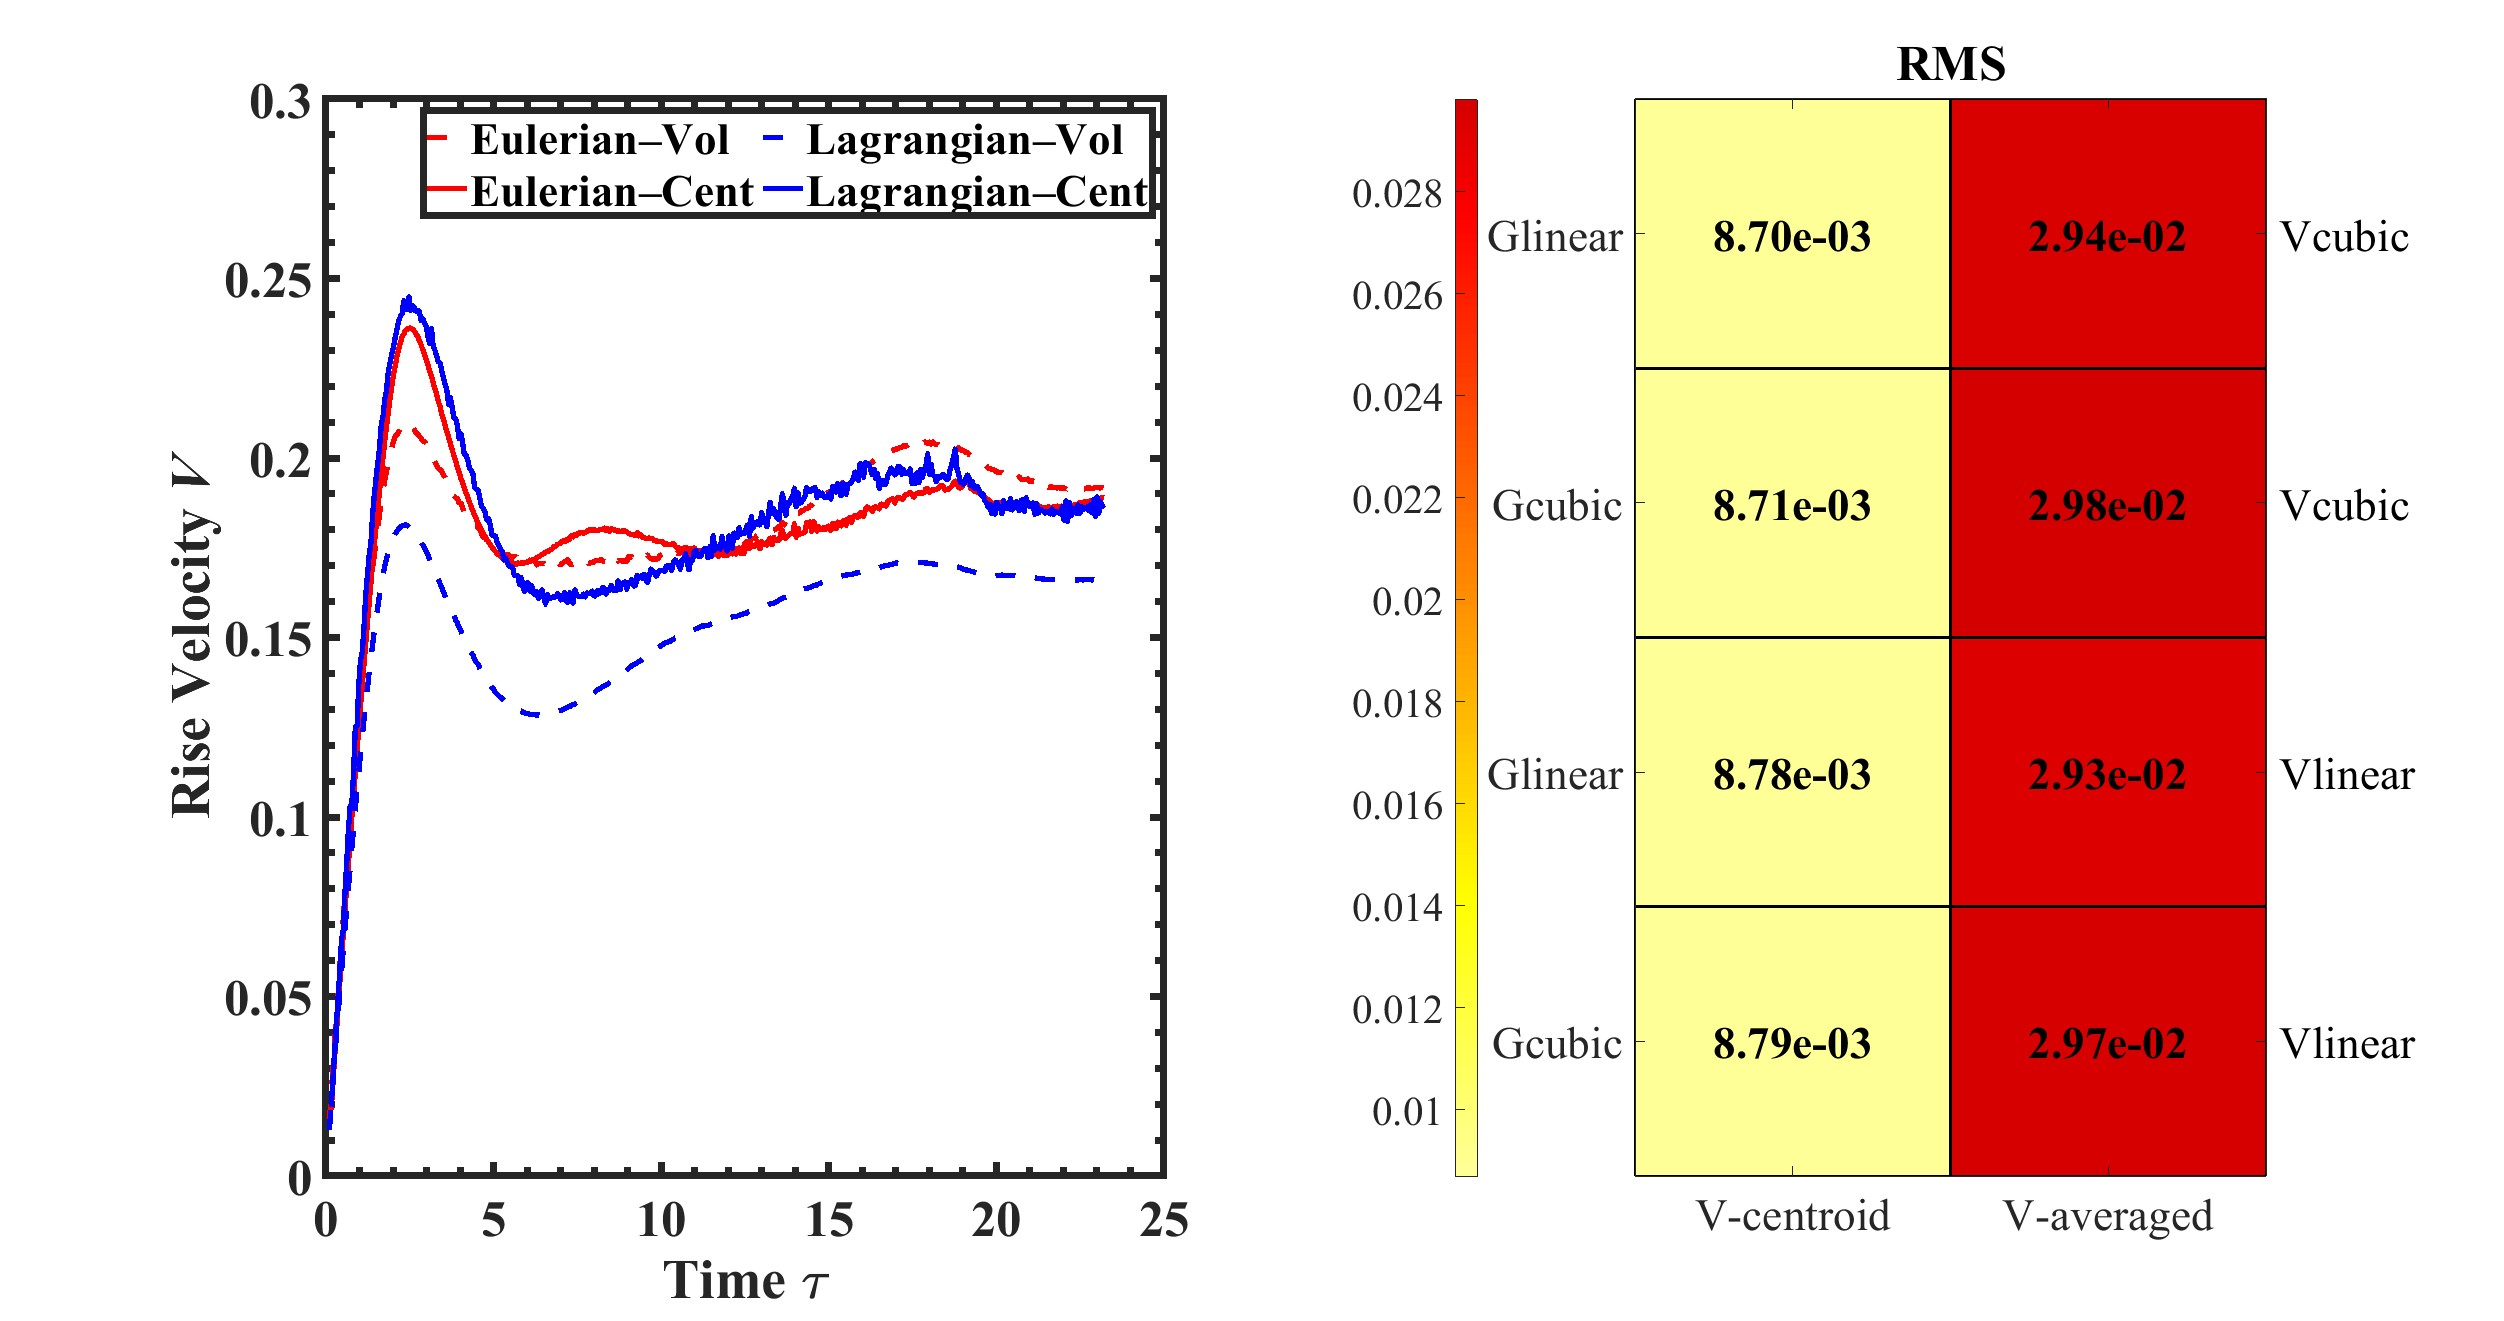
\includegraphics[width=\textwidth]{Fig1a.jpg}
		\caption{%
			Scattered Lagrangian data.
			\textbf{Left:} Temporal evolution of the non-dimensional rise velocity,
			comparing the Eulerian reference (red) with the scattered Lagrangian
			estimate (blue) for the case with linear interpolation scheme for velocity and gas volume fraction. Solid lines
			correspond to the centroid-based method; dashed lines to the
			volume-averaged method.
			\textbf{Right:} RMS error heatmap across all four interpolation
			combinations.  Rows indicate the gas fraction interpolation scheme and
			columns distinguish between centroid-based and volume-averaged methods.
			Labels on the right margin identify the velocity interpolation scheme.}
		\label{fig:fig1a}
	\end{figure}
	
	% --- Figure 1b: Scattered field profiles ---
	\begin{figure}[ht]
		\centering
		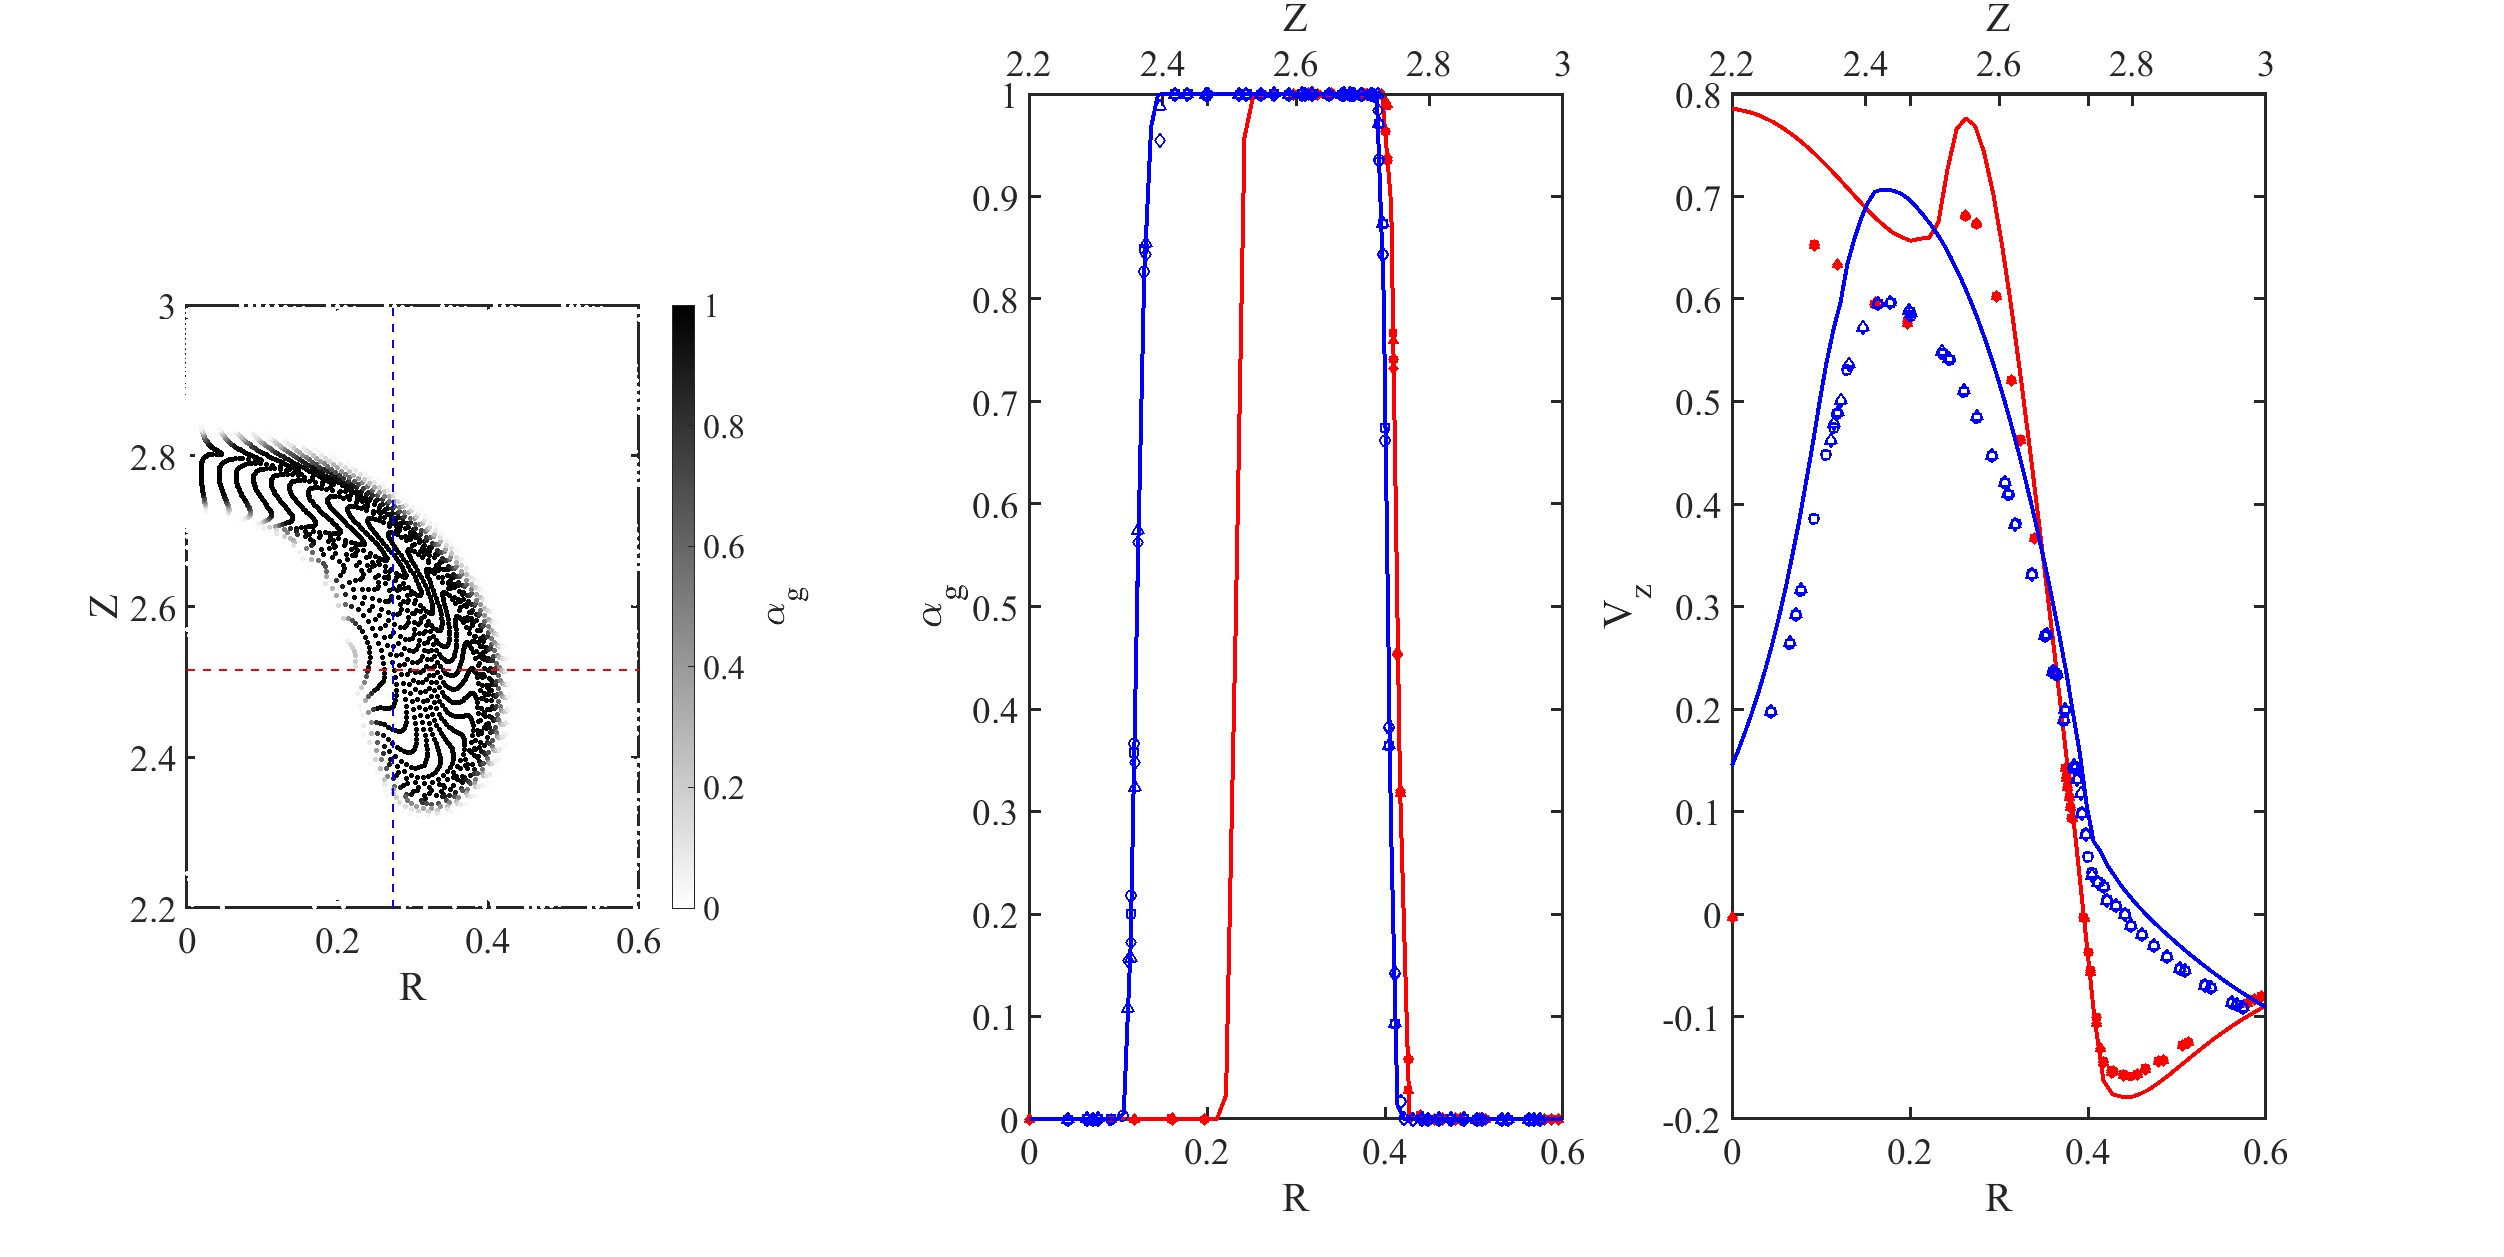
\includegraphics[width=\textwidth]{Fig1b.jpg}
		\caption{%
			Scattered Lagrangian data at $\tau \approx 6.3$.
			\textbf{Left:} Scatter plot of Lagrangian particle positions coloured by
			the gas volume fraction $\alphag$; dashed lines indicate the horizontal
			(red, $r$-direction) and vertical (blue, $z$-direction) cut-lines.
			\textbf{Middle:} Gas fraction profiles along the two cut-lines:
			Eulerian reference (solid lines) versus scattered Lagrangian values
			(markers) for all four interpolation combinations.
			Red denotes the $r$-direction (bottom axis); blue denotes the
			$z$-direction (top axis).
			\textbf{Right:} Corresponding axial velocity profiles.
			The larger scatter in velocity compared with gas fraction confirms that
			$\Vz$ interpolation is the dominant error source.}
		\label{fig:fig1b}
	\end{figure}
	
	% --- Figure 2a: Interpolated rise velocity + RMS heatmap ---
	\begin{figure}[ht]
		\centering
		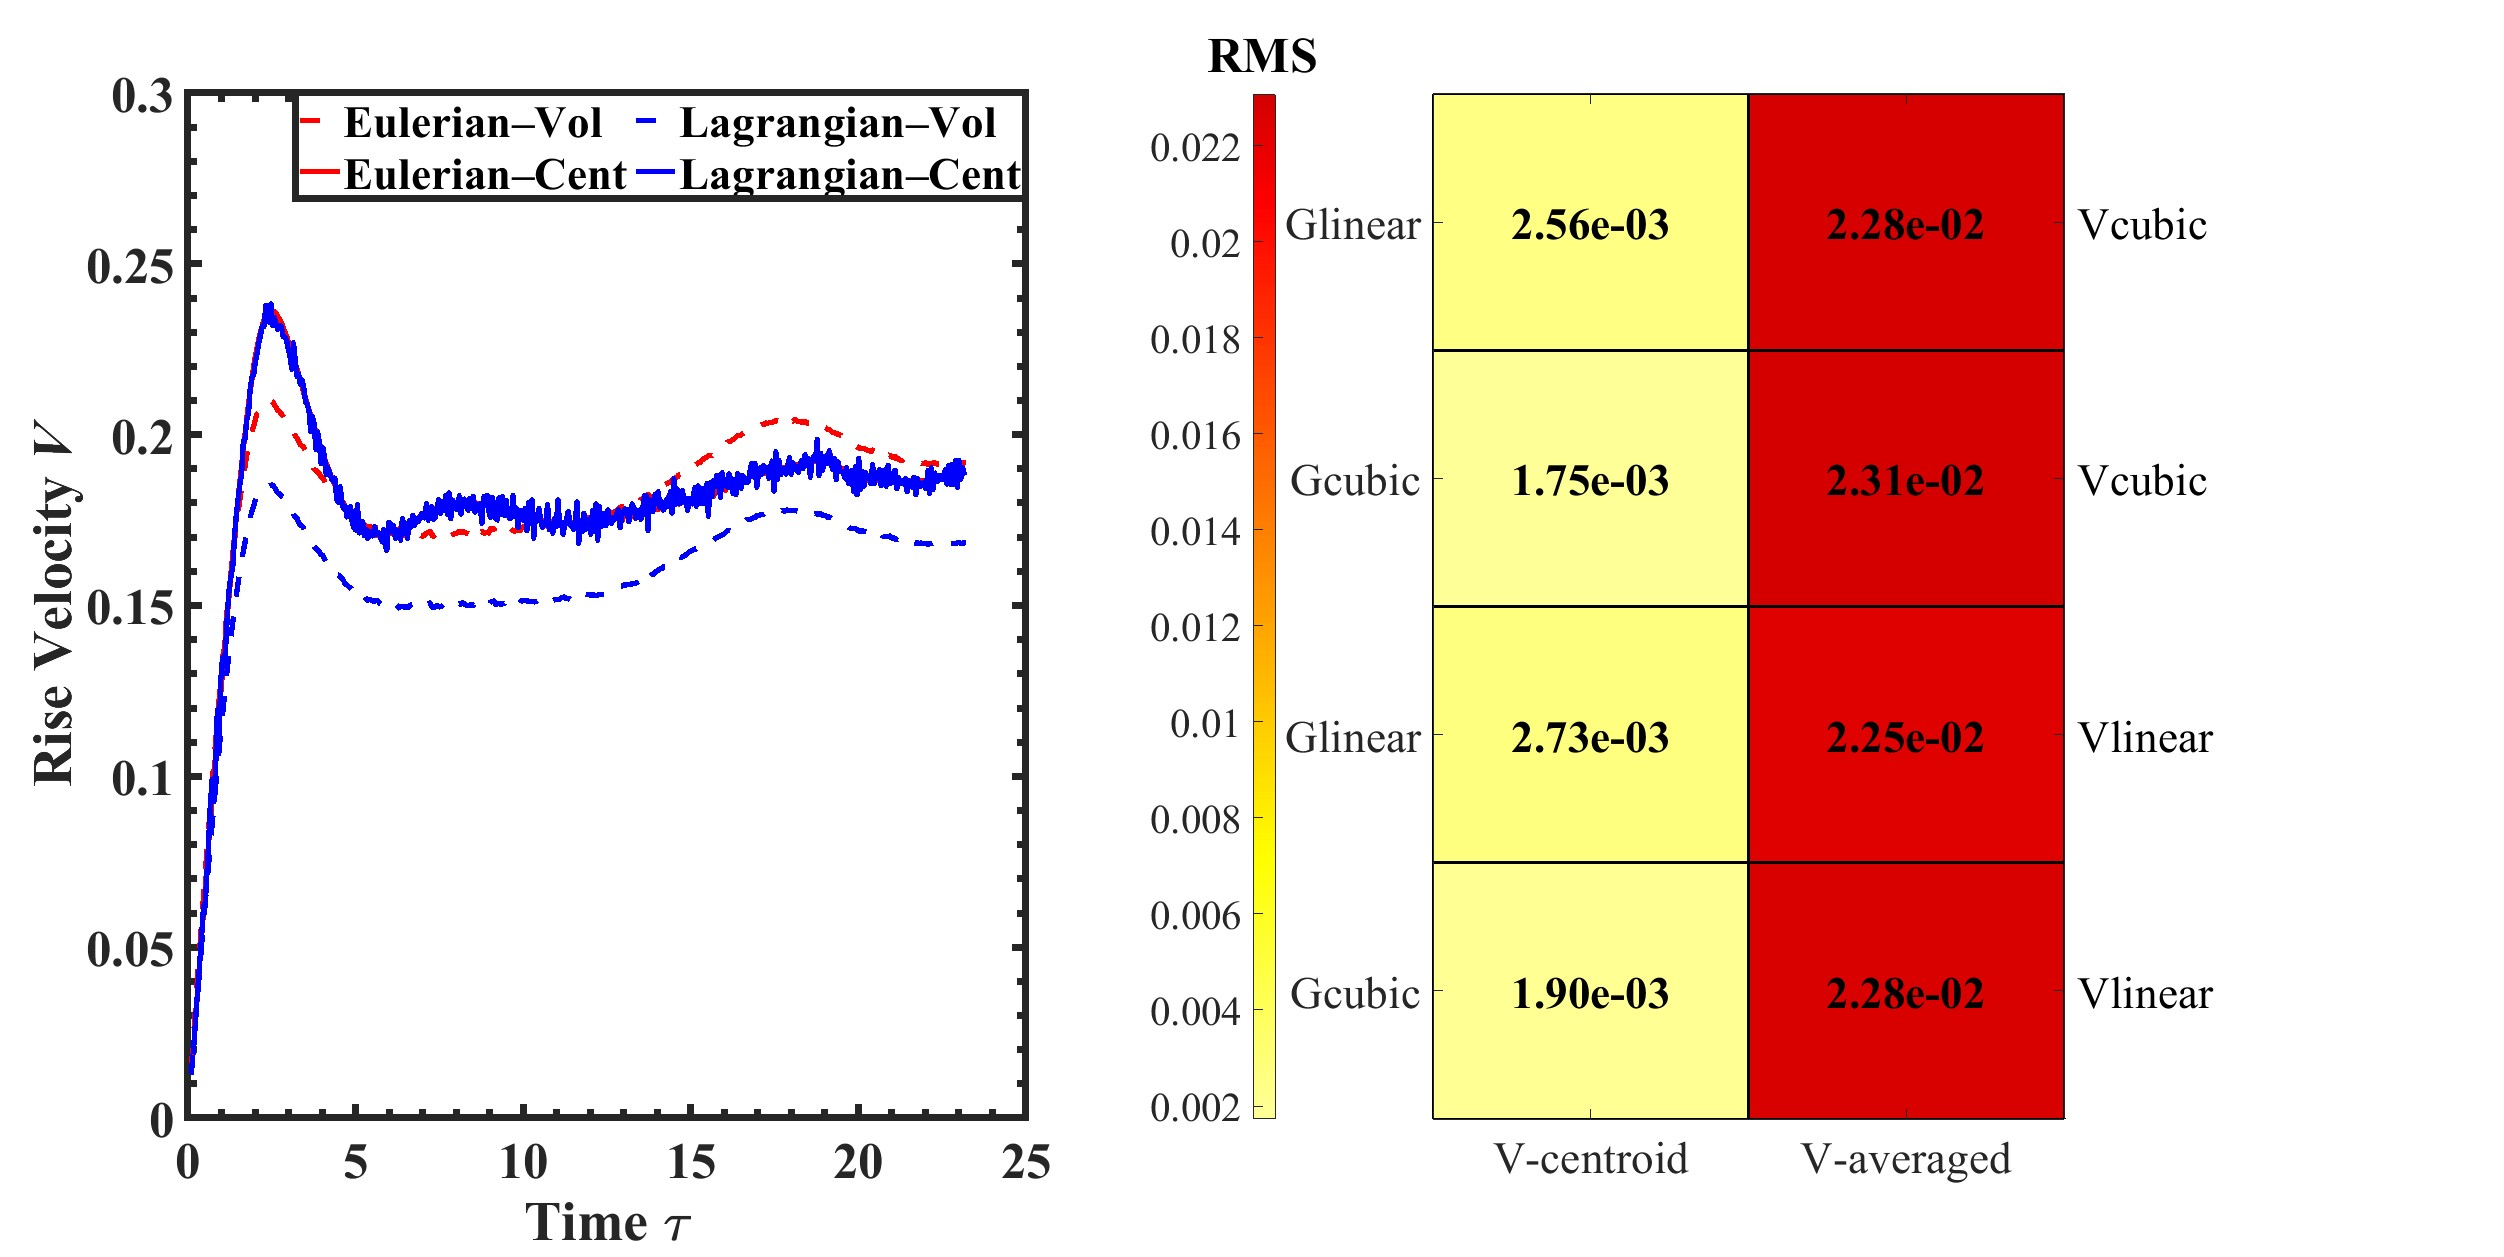
\includegraphics[width=\textwidth]{Fig2a.jpg}
		\caption{%
			Re-interpolated Lagrangian data.
			\textbf{Left:} Temporal evolution of the non-dimensional rise velocity
			after re-interpolation.  The centroid-based Lagrangian estimate (blue
			solid) now nearly overlaps the Eulerian reference (red solid), while the
			volume-averaged estimate (blue dashed) remains offset.
			\textbf{Right:} RMS error heatmap.  Centroid-based errors have decreased
			by a factor of 3--5 compared with \cref{fig:fig1a}; volume-averaged
			errors show only modest improvement.}
		\label{fig:fig2a}
	\end{figure}
	
	% --- Figure 2b: Interpolated field profiles ---
	\begin{figure}[ht]
		\centering
		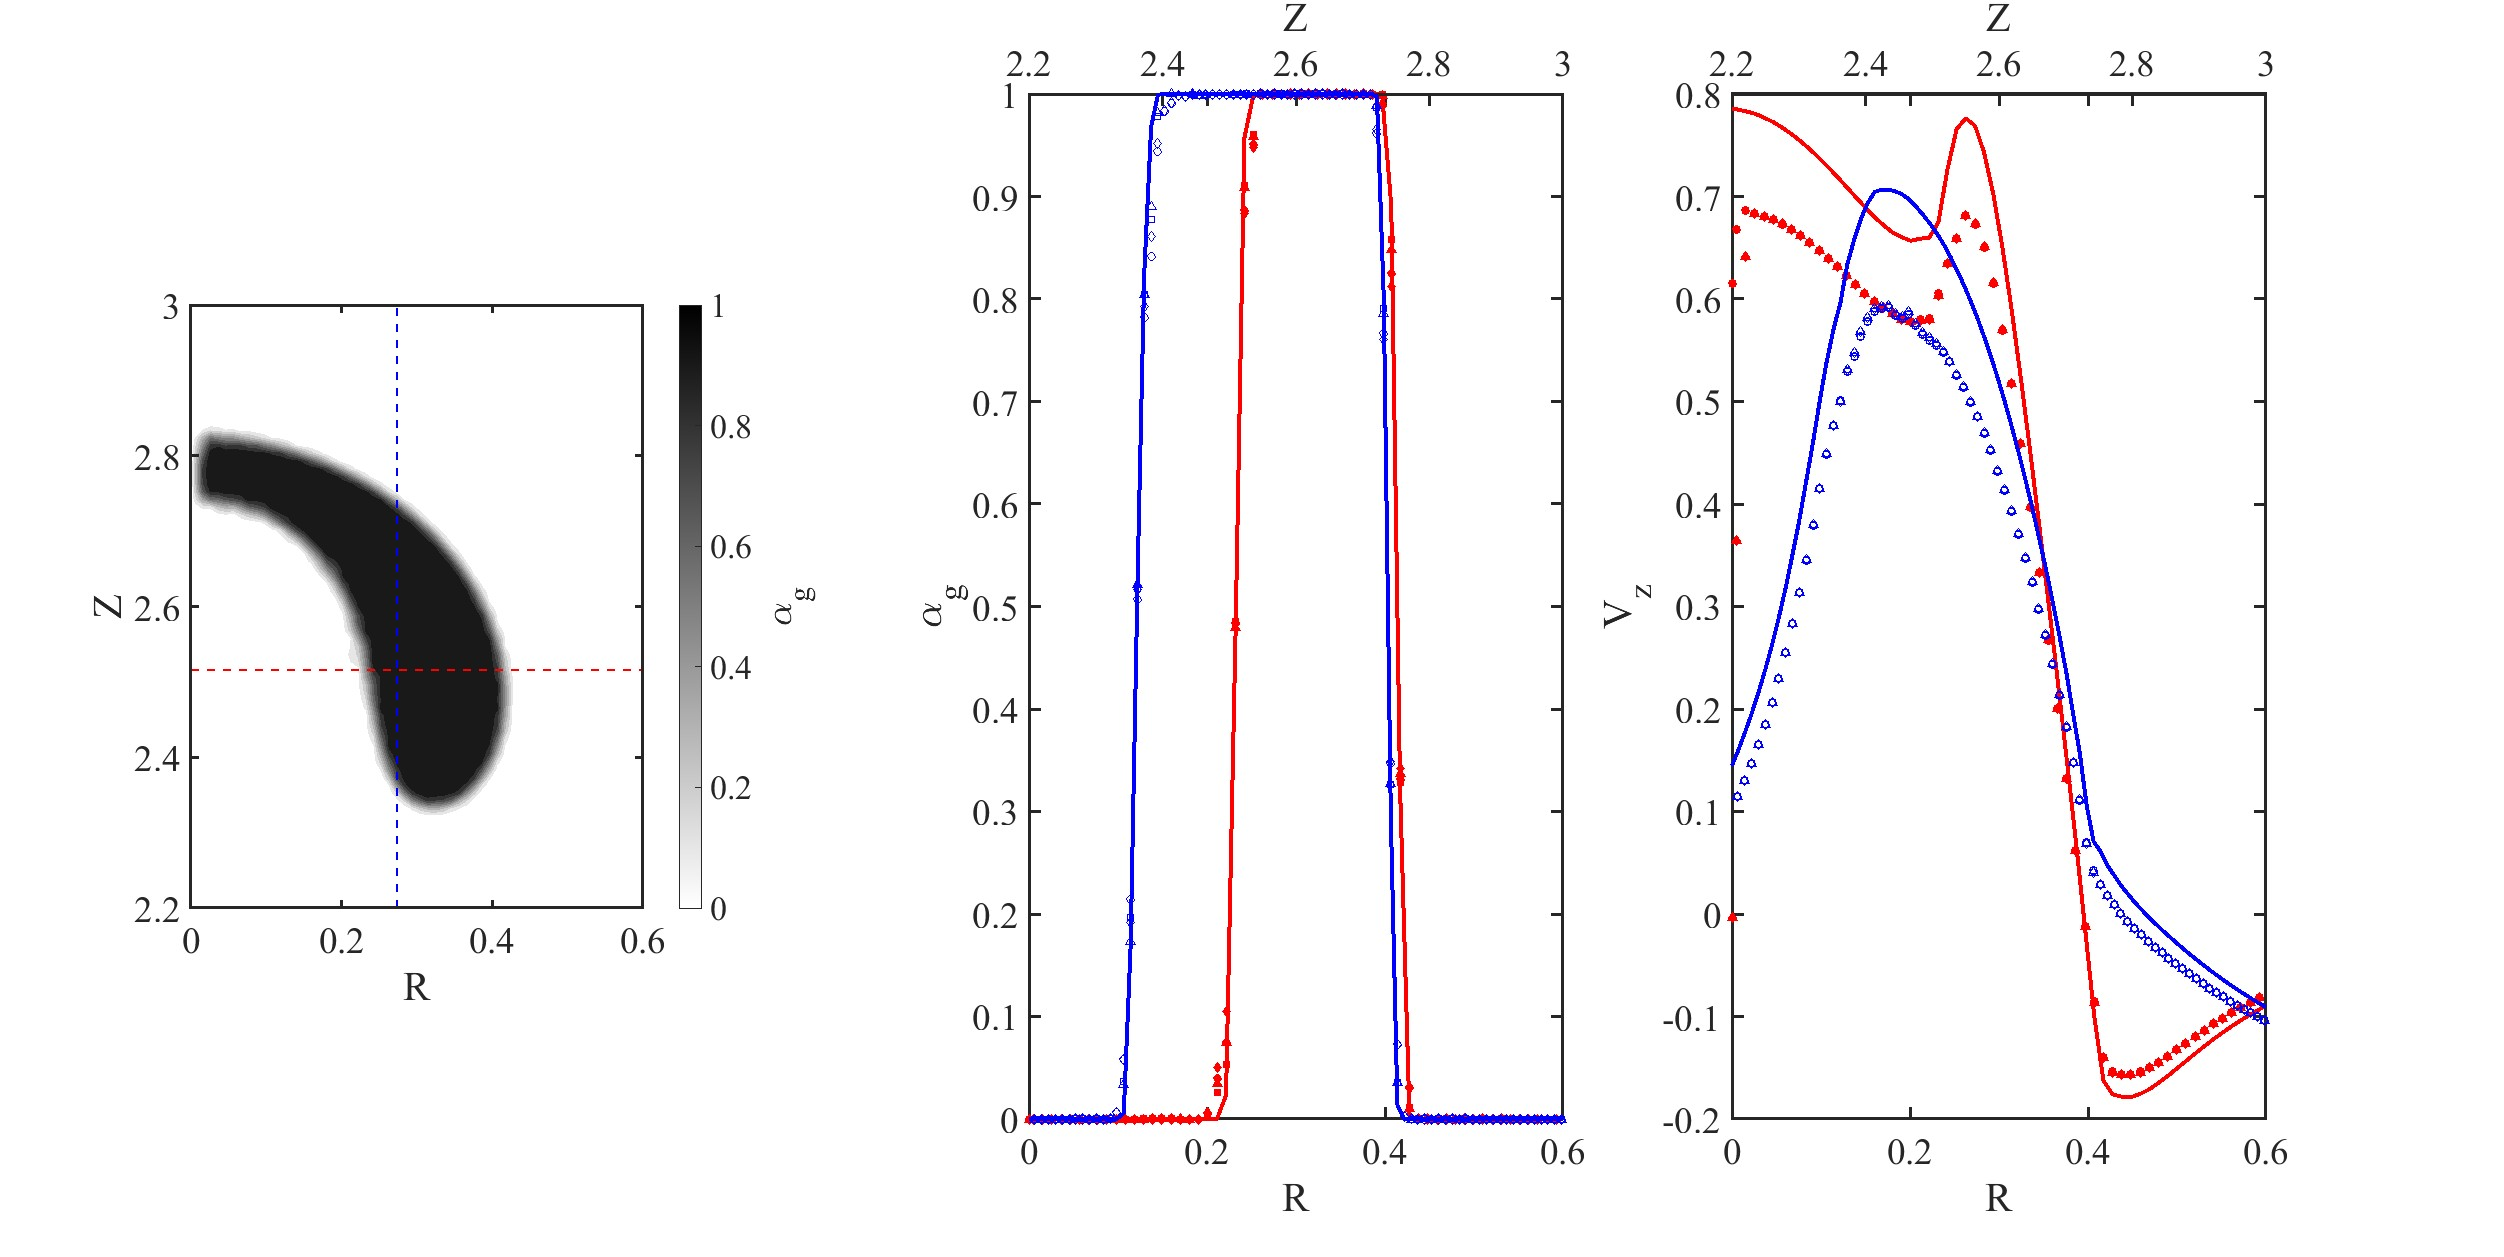
\includegraphics[width=\textwidth]{Fig2b.jpg}
		\caption{%
			Re-interpolated Lagrangian data at $\tau \approx 6.3$.
			\textbf{Left:} Contour plot of the re-interpolated gas fraction field
			for the first Lagrangian case, with diagnostic cut-lines indicated.
			\textbf{Middle:} Re-interpolated gas fraction profiles along the
			cut-lines, now smooth and closely matching the Eulerian reference.
			\textbf{Right:} Re-interpolated velocity profiles.  While smoother
			than the scattered counterpart (\cref{fig:fig1b}), deviations from the
			Eulerian reference persist, particularly inside the bubble.}
		\label{fig:fig2b}
	\end{figure}
	
	% =========================================================================
	\section{Results and discussion}\label{sec:results}
	% =========================================================================
	
	\subsection{Spectral compressibility}\label{sec:compress}
	
	The central claim of this work is that a change of reference frame ---
	from the fixed Eulerian (E) frame to the Lagrangian (L) or
	moving-Eulerian (ME) frame --- concentrates the energy of the snapshot
	matrix into fewer POD modes, thereby making the data more amenable to
	low-rank approximation.
	To quantify this effect we introduce three complementary metrics
	evaluated on the POD singular values
	$\sigma_1 \geq \sigma_2 \geq \cdots \geq \sigma_N$
	obtained from the snapshot matrix $\mathbf{X}$.
	
	\paragraph{Residual energy.}
	The fraction of total energy \emph{not} captured by the leading $r$
	modes,
	\begin{equation}\label{eq:Eres}
		E_{\mathrm{res}}(r)
		= 100 \left(1 - \frac{\sum_{i=1}^{r}\sigma_i^{2}}
		                      {\sum_{i=1}^{N}\sigma_i^{2}}\right)
		\qquad [\%],
	\end{equation}
	is plotted on a logarithmic ordinate so that differences between
	frames remain visible even when both are close to machine precision.
	
	\paragraph{99\,\%-energy rank.}
	The smallest rank $r_{99}$ satisfying
	\begin{equation}\label{eq:r99}
		\frac{\sum_{i=1}^{r_{99}}\sigma_i^{2}}
		     {\sum_{i=1}^{N}\sigma_i^{2}} \geq 0.99
	\end{equation}
	provides a single integer that summarises how many modes are needed to
	represent 99\,\% of the snapshot energy.
	
	\paragraph{Normalised spectral entropy.}
	Define the mode-energy fractions
	$p_i = \sigma_i^{2}/\sum_j \sigma_j^{2}$
	and the Shannon entropy of that distribution,
	\begin{equation}\label{eq:Hnorm}
		H_{\mathrm{norm}}
		= -\frac{\sum_{i=1}^{N} p_i \ln p_i}{\ln N}
		\;\in [0,\,1].
	\end{equation}
	A value of $H_{\mathrm{norm}}=0$ corresponds to all energy in a single
	mode; $H_{\mathrm{norm}}=1$ to a uniform distribution.  Unlike $r_{99}$,
	the entropy accounts for the \emph{shape} of the entire spectrum and is
	therefore sensitive to how broadly energy is spread across all modes,
	not just the threshold at which a fixed percentage is reached.
	
	\Cref{fig:spectral} collects all three metrics for two Reynolds numbers
	($\mathrm{Re}=20$ and $\mathrm{Re}=100$), two physical quantities (gas
	volume fraction and velocity), and three reference frames (E, L, ME).
	For the Lagrangian frame an additional curve corresponding to the
	particle-position field is included, since positions are tracked natively
	in that frame and their temporal derivative recovers the velocity.
	
	\paragraph{Gas volume fraction.}
	Across both Reynolds numbers the frame change produces a dramatic
	reduction in spectral complexity.  At $\mathrm{Re}=20$ the E-frame
	requires $r_{99}=49$ modes, whereas the L-frame needs only 9 and the
	ME-frame only 5.  The corresponding normalised entropies drop from
	$H_{\mathrm{norm}}=0.43$ (E) to $0.23$ (L) and $0.12$ (ME).
	At $\mathrm{Re}=100$ the trend is preserved: the E-frame $r_{99}$
	rises to 83, while the L- and ME-frames remain at 15 and 19,
	respectively.  The residual-energy curves (\cref{fig:spectral},
	left column) confirm that the L- and ME-frame curves decay orders of
	magnitude faster than the E-frame curve, reflecting the removal of
	the dominant translational dynamics from the snapshot data.
	
	\paragraph{Velocity field.}
	The velocity results reveal a subtler picture.  While $r_{99}$ still
	decreases when switching frames (from 10 to 8 to 3 at $\mathrm{Re}=20$;
	from 21 to 14 to 10 at $\mathrm{Re}=100$), the normalised entropy of
	the L-frame velocity is nearly indistinguishable from that of the
	E-frame ($H_{\mathrm{norm}}\approx 0.28$ at $\mathrm{Re}=20$ and
	$\approx 0.27$--$0.30$ at $\mathrm{Re}=100$).
	This indicates that, although fewer modes cross the 99\,\% threshold,
	the residual spectral energy is redistributed rather than eliminated:
	the Lagrangian transformation removes the leading translational
	component but does not simplify the remaining wake structures.
	Only the moving-Eulerian frame, which additionally removes
	the mean-flow advection, achieves a substantial entropy reduction
	($H_{\mathrm{norm}}=0.13$ at $\mathrm{Re}=20$; $0.22$ at
	$\mathrm{Re}=100$).
	
	\paragraph{Summary.}
	For both quantities and both Reynolds numbers the spectral metrics
	consistently demonstrate that a change of reference frame ---
	particularly to the moving-Eulerian frame --- concentrates the
	snapshot energy into markedly fewer modes.  This concentration is
	independent of the decomposition method used (the singular values
	analysed here come from the POD, but the same snapshot matrix feeds
	both POD and DMD), and it is this improved compressibility that
	underpins the accuracy gains in low-rank reconstructions.
	
	% --- Figure 3: Spectral compressibility ---
	\begin{figure}[t]
		\centering
		\includegraphics[width=\textwidth]{Fig3_spectral.pdf}
		\caption{%
			Spectral compressibility of the snapshot matrices for
			$\mathrm{Re}=20$ and $\mathrm{Re}=100$.
			\textbf{Left column:} Residual energy $E_{\mathrm{res}}(r)$
			(log scale); solid lines denote $\mathrm{Re}=100$, dashed lines
			$\mathrm{Re}=20$.
			\textbf{Middle column:} 99\,\%-energy rank $r_{99}$ (bar chart);
			solid bars for $\mathrm{Re}=100$, hatched bars for $\mathrm{Re}=20$.
			\textbf{Right column:} Normalised spectral entropy
			$H_{\mathrm{norm}}$ (bar chart, same hatching convention).
			\textbf{Top row:} Gas volume fraction.
			\textbf{Bottom row:} Velocity (and Lagrangian positions).
			Colours: Eulerian (black), Lagrangian (blue),
			moving-Eulerian (green).}
		\label{fig:spectral}
	\end{figure}
	
	
\end{document}
